%Paul E. West

%\documentclass[xcolor=svgnames]{beamer}
\documentclass{beamer}
\usepackage[boxed,vlined,figure]{algorithm2e}

%\usecolortheme[named=FireBrick]{structure}
%\usecolortheme[named=black]{structure}
%\usecolortheme{beetle}
%\usecolortheme{beaver}
%\usecolortheme{crane}
%\usecolortheme{dolphin}
%\usecolortheme{dove}
%\usecolortheme{fly}
%\usecolortheme{lily}
\usecolortheme{orchid}
%\usecolortheme{rose}
%\setbeamercolor{background canvas}{bg=Gold!25}
%\setbeamercolor{background canvas}{bg=Black!100}
%\setbeamercolor{foreground}{bg=Gold!25}
%\setbeamercolor{normal text}{fg=green,bg=black}
%\setbeamercolor*{palette primary}{use=structure,fg=green,bg=black}

\mode<presentation>{
    \usetheme{Darmstadt}
    \setbeamercovered{invisible}
    %\setbeamercovered{transparent}
    \setbeamercolor*{palette primary}{use=structure,fg=white,bg=blue}
    \setbeamercolor*{palette secondary}{use=structure,fg=white,bg=blue}
    \setbeamercolor*{palette tertiary}{use=structure,fg=white,bg=blue}
}

\usepackage[english]{babel}
\usepackage[latin1]{inputenc}
\usepackage{times}
\usepackage[T1]{fontenc}
%\usepackage{epsfig}
\usepackage{ulem}
\usepackage{color,soul}

\usepackage{graphicx}
\usepackage{amssymb}
\usepackage{url,hyperref}
\definecolor{beamer@blendedblue}{rgb}{1,.6,.2}
%\usepackage{tikz}
%\usetikzlibrary{shapes}
%\usetikzlibrary{arrows}
%\tikzstyle{block}=[draw opacity=0.7, line width=1.4cm]
\usepackage{listings}
\lstset{language=C++}
\lstset{showspaces=false}
\lstset{showstringspaces=false}
\lstset{tabsize=4}
\lstset{basicstyle=\tiny}


%\usecolortheme[overlystylish]{albatross}
%\usecolortheme[]{lily}
%\usecolortheme[]{albatross}
%\usecolortheme[]{orchid}
%\setbeamercolor{normal text}{fg=green!10}

\title{CSCI 315: Data Structures \\ C++ Testing, Pointers, and OOP}
\author{Paul E. West, PhD}

\institute{
  Department of Computer Science\\
  Charleston Southern University
}

\subject{Software Programming}
%\keywords{Performance Counters, Multicore}

%\pgfdeclareimage[height=1.0cm]{university-logo}{../imgs/csu-logo}
\pgfdeclareimage[height=0.75cm]{university-logo}{../imgs/csu-logo}
%\pgfdeclareimage[height=0.50cm]{university-logo}{../imgs/csu-logo}
\logo{\pgfuseimage{university-logo}}

\begin{document}

\begin{frame}
  \titlepage
\end{frame}

\section{Overview}
\subsection{}

\begin{frame}{}
\begin{itemize}
\item Objects in C++ share many similarities with Java, but are considered more powerful:
\begin{itemize}
\item They can be created on the stack.
\item C++ allows multiple inheritance.
\begin{itemize}
\item no need for the interface keyword.
\end{itemize}
\item Templates act like generics, except they are a compile time construct, not run time.
\end{itemize}
\item Remember, C++ is compiled to machine code, Java compiles to byte code!
\end{itemize}
%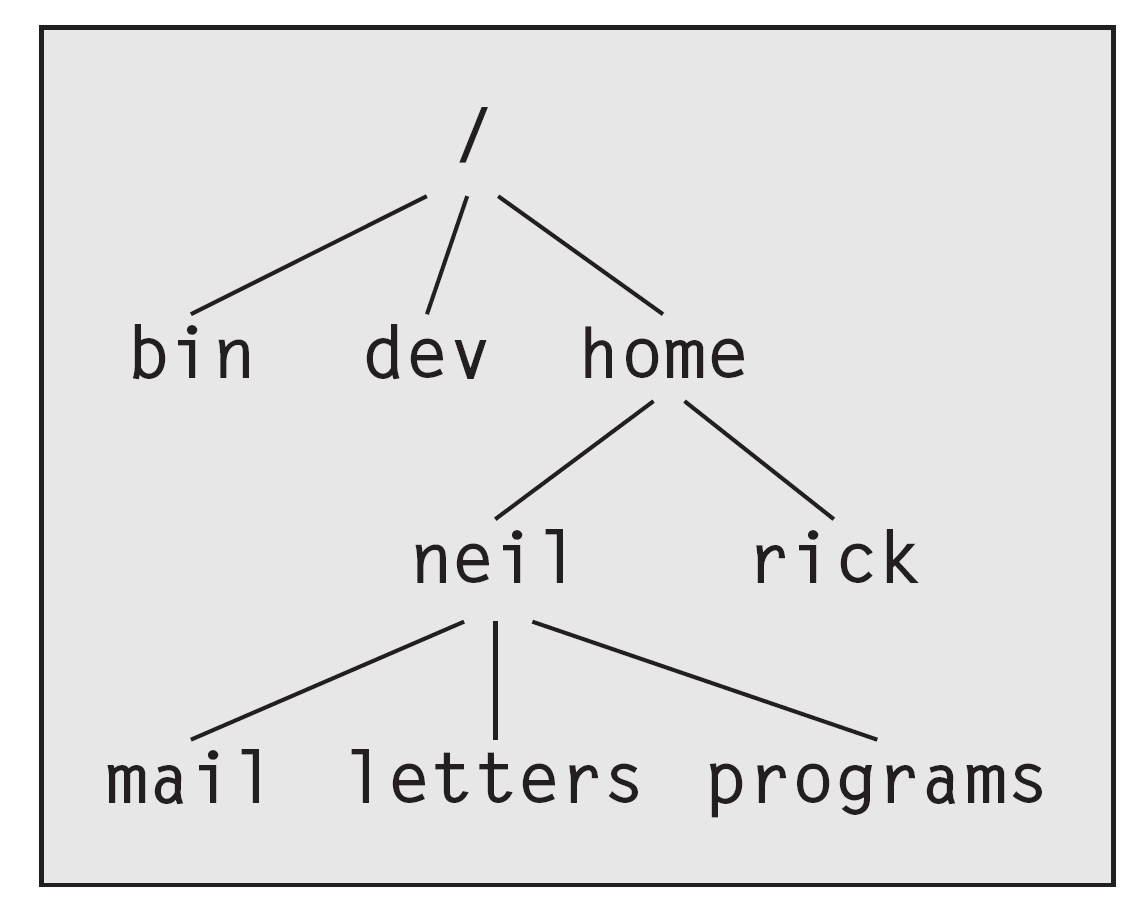
\includegraphics[width=1.0\textwidth]{../imgs/simple-directories.png}
\end{frame}

\section{Testing}
\subsection{}

\begin{frame}{Testing}
\underline{\textbf{\textit{Testing will make you more productive.}}} \\
This means you will spend less time working on problems because you will increase you chances of getting it right the first time AND virtually never make the same mistake twice.
\end{frame}

\begin{frame}{Warning}
\begin{itemize}
\item Proven Fact: A computer program cannot sufficient generate test cases for you code.
\item When I say proven, I mean Turing wrote a proof that shows beyond the shadow of a doubt that it is impossible for a computer to determine if a program halts.
\item If we don't know if it halts how can we test?
\item This is your job, and an advantage you have over the machines.
\end{itemize}
\end{frame}

\begin{frame}{Unit Test}
\begin{itemize}
\item For this class Unit testing is sufficient.
\item There are many other forms of testing, but this class focuses on (relatively) small units of code.
\item There are numerous Unit Testing tools, but no de facto for C++
\begin{itemize}
\item Unlike Java's JUnit
\end{itemize}
\item I have chosen CXXTestGen for this class.
\begin{itemize}
\item It is the simplest which still providing sufficient robustness.
\end{itemize}
\end{itemize}
\end{frame}

\begin{frame}[fragile]{CXX Test Gen}
\begin{itemize}
\item Make sure you have it installed:
\begin{itemize}
\item \# apt install cxxtestgen
\end{itemize}
\item Simple test case:
\end{itemize}
\begin{lstlisting}
#include <cxxtest/TestSuite.h>
#include <limits.h>
#include <stdio.h>

int add(int a, int b) {
    return a + b;
}

class MyTestSuite1 : public CxxTest::TestSuite {
    public:
        void test1(void) {
            /* Fill in some test cases here for cxx test gen */
            TS_ASSERT(add(1, 2) == 3);
        }
};

\end{lstlisting}
\end{frame}

\begin{frame}{Running The Test}
\begin{enumerate}
\item First we generate the test code using cxxtestgen: \\
\$ cxxtestgen --runner=ErrorPrinter -o test-runner.cpp simple-test.cpp 
\item Then we compile the code: \\
\$ g++ test-runner.cpp -o test-runner
\item Then we run! \\
\$ ./test-runner
\end{enumerate}
\begin{itemize}
\item Keep in mind that we will want to test code in other files.
\item So, we need to include that file in \#2, for example if we had a sum.cpp, then \#2 would be:\\ 
\$ g++ sum.cpp test-runner.cpp -o test-runner
\item You make add optimization and profiling if desired.
\end{itemize}
\end{frame}


\section{Pointers}
\subsection{}

\begin{frame}{Overview}
\begin{itemize}
\item As I said, in C++ a pointer can point to anything (well anything that is pointable!)
\end{itemize}
\end{frame}

\begin{frame}{Stack Pointer}
\begin{itemize}
\item int *a;
\begin{itemize}
\item declare a variable 'a' that stores the memory address of where an integer resides.
\end{itemize}
\item int b = 32; \\
a = \&b;
\item the \& symbol calculates the memory address of the following variable.
\item So the above declares 'b' on the stack, sets 'b' to 32, then stores the memory address of 'b' in 'a'.
\item *a = 64;
\item In this instance the *, mean go to where 'a' is pointing and store 32 there.
\item Since 'a' is pointing to 'b', b now has 64.
\end{itemize}
\end{frame}

\begin{frame}{Heap Pointer}
\begin{itemize}
\item int *a = new int;
\item This reads, create a variable 'a' on the stack that will store the memory address of an integer.  Next allocate an int in memory and store the memory address of that int in 'a'.
\item You can manipulate the new int just like before.
\item Although, since the integer is on the heap, you must deallocate!
\begin{itemize}
\item delete a;
\end{itemize}
\end{itemize}
\end{frame}

\begin{frame}{Arrays/Pointer Arithmetic}
\begin{itemize}
\item int ary[100];\\
int *a = ary;
\item first line creates an array of 100 integers on the stack.
\item second line creates a pointer to the array.  Notice we didn't need the \&!
\item *(a+10) = 50; Is the same as:\\
ary[10] = 50!
\end{itemize}
\end{frame}

\begin{frame}{Casting}
\begin{itemize}
\item C++ is incredibly powerful, because of casting.\\
int b = 300; \\
int *a = \&b; \\
double *d = (double*)a; \\
*d = 3.14159;
\item Yes, that is legal. 
\item What is the value of b?
\item <2-> Undefined!
\end{itemize}
\end{frame}

\begin{frame}{There is more}
\begin{itemize}
\item Pointers can point to other things:
\begin{itemize}
\item functions
\item other pointers
\item Arrays
\item objects
\end{itemize}
Lastly, void * means I'm creating a pointer to something.
\end{itemize}
\end{frame}

\section{C++ vs Java OOP}
\subsection{}

\begin{frame}{Class Organization}
\begin{itemize}
\item Enforced through access keywords
\begin{itemize}
\item public: for interface
\item private: to make implementation inaccessible
\item protected: access for subclasses only
\end{itemize}
\item In Java
\begin{itemize}
\item each member is prefixed with a keyword
\item another access level:  package-access
\end{itemize}
\item In C++
\begin{itemize}
\item public, private, and protected sections
\item friend keyword used to break encapsulation (don't use!)
\end{itemize}
\end{itemize}
%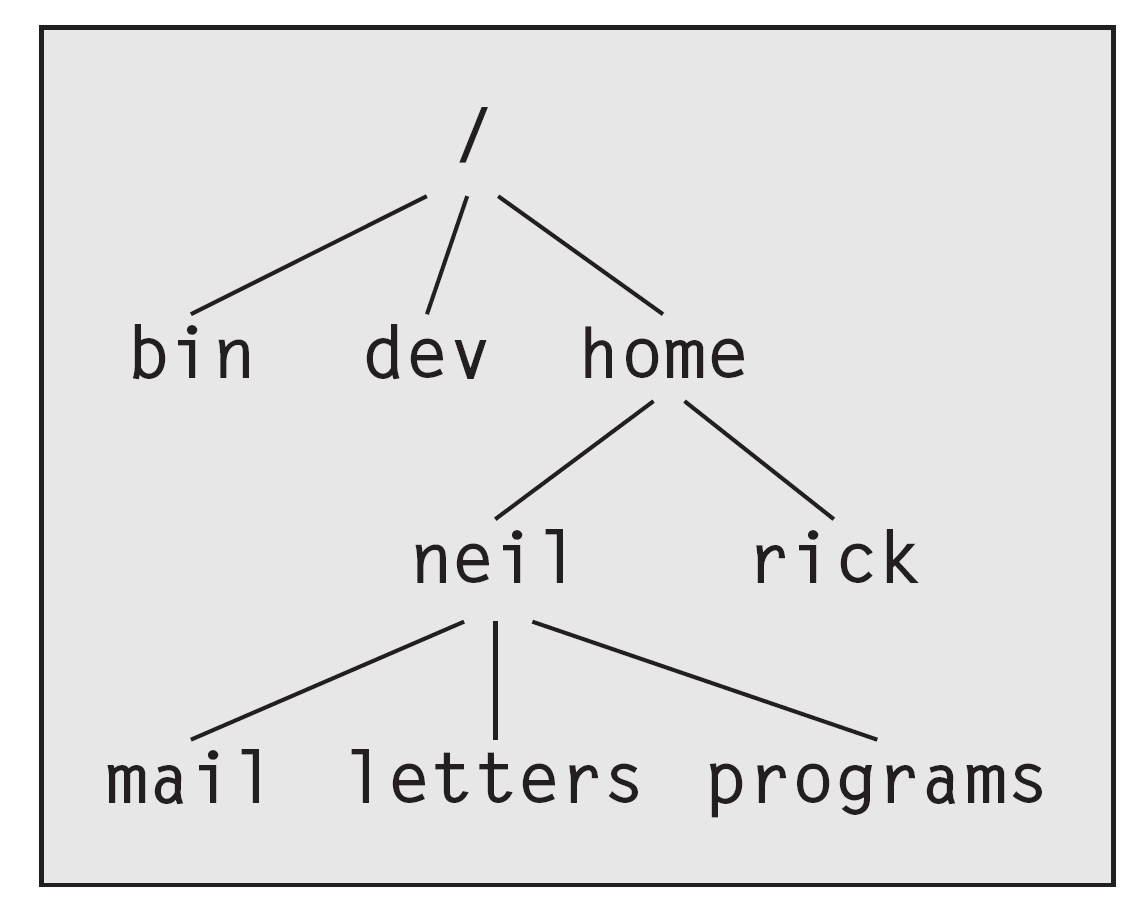
\includegraphics[width=1.0\textwidth]{../imgs/simple-directories.png}
\end{frame}

\begin{frame}{Inheritance}
\begin{itemize}
\item Feature that allows a class to be defined based on another class
\begin{itemize}
\item methods and attributes are inherited
\end{itemize}
\item Java and C++ difference
\begin{itemize}
\item Java:  public class A extends B { }
\item C++:  class A: public B { }; \\
(different types of inheritance)
\end{itemize}
\item Multiple inheritance possible in C++, not in Java
\item But in Java, one may implement several interfaces
\end{itemize}
%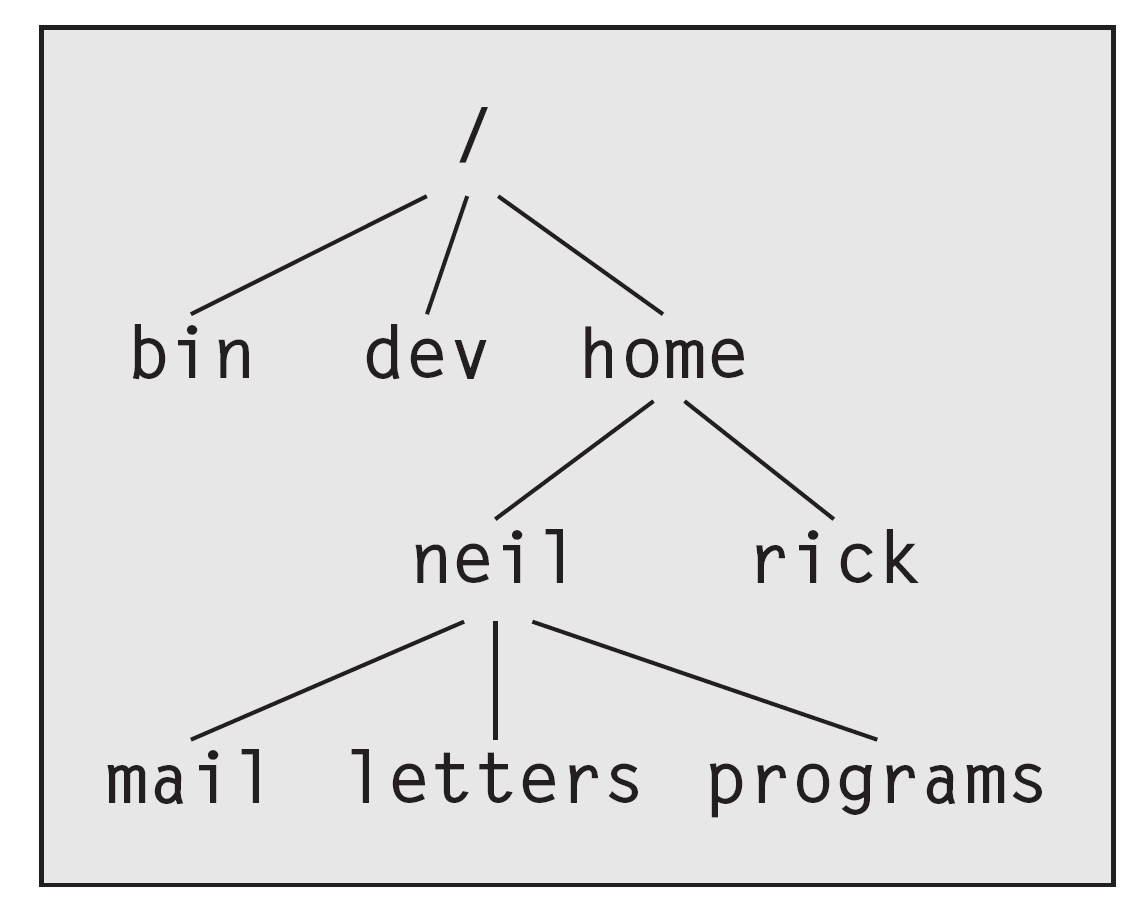
\includegraphics[width=1.0\textwidth]{../imgs/simple-directories.png}
\end{frame}

\begin{frame}{Parametric Polymorphism}
\begin{itemize}
\item We will get to later...
\end{itemize}
%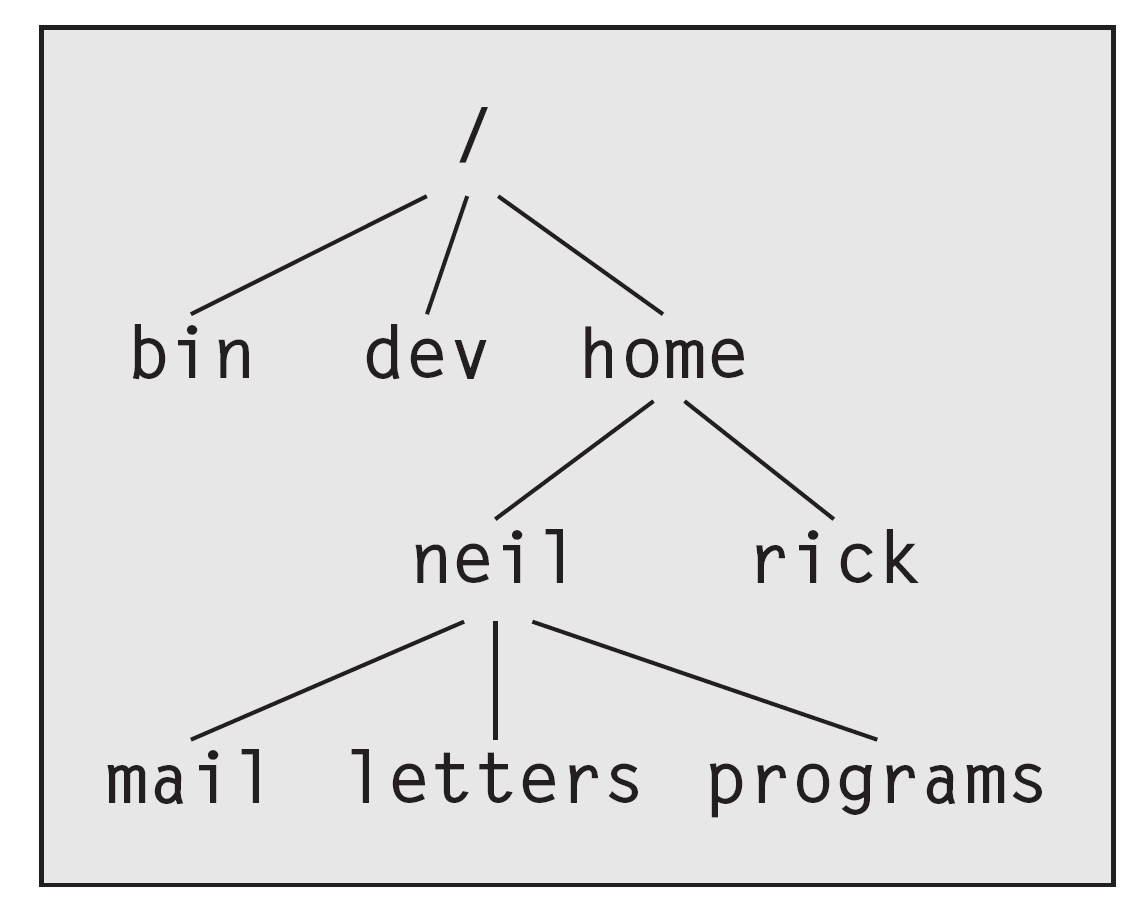
\includegraphics[width=1.0\textwidth]{../imgs/simple-directories.png}
\end{frame}

\begin{frame}{Pointers}
\begin{itemize}
\item In Java a pointer was called a reference to an object:
\begin{itemize}
\item String str = new String("Hello!");
\end{itemize}
\item In C++ a pointer stores the memory location of something else
\item For objects:
\begin{itemize}
\item std::string *str = new std::string("Hello!);
\end{itemize}
\end{itemize}
%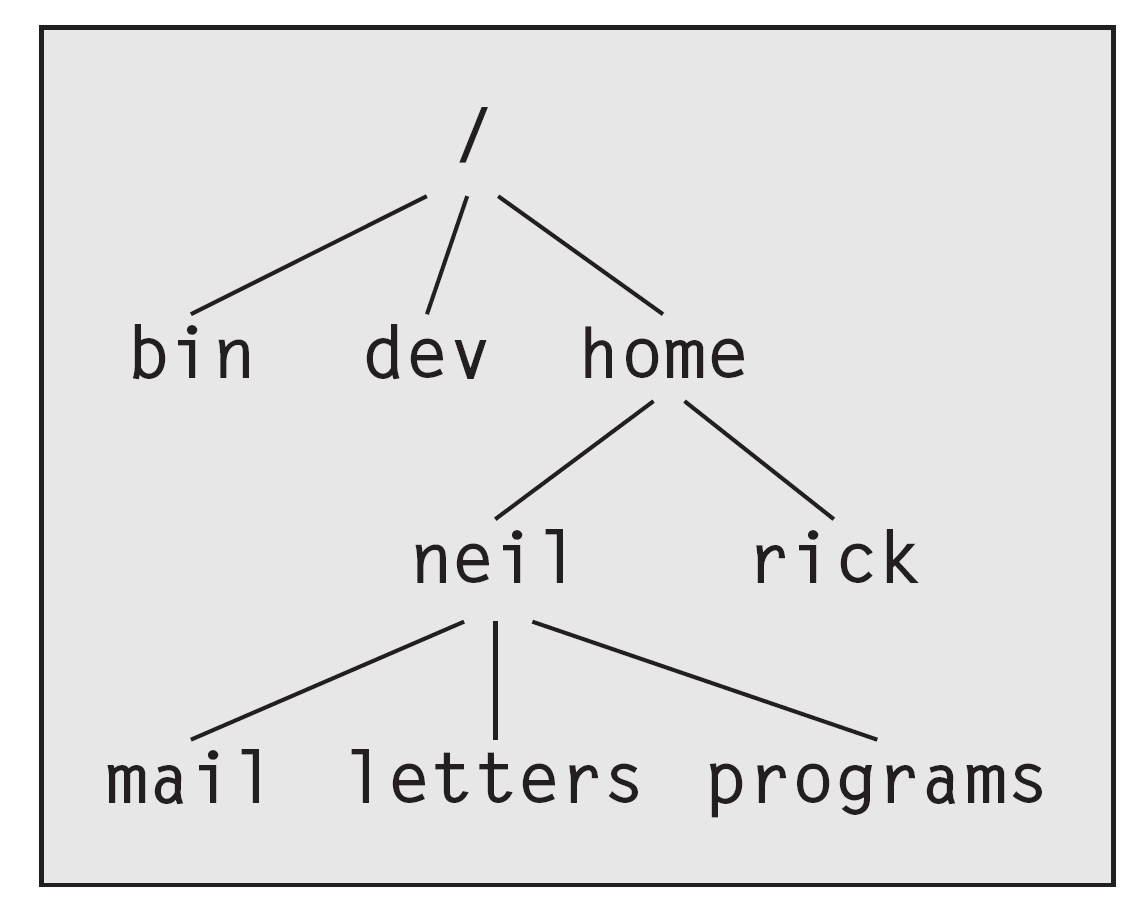
\includegraphics[width=1.0\textwidth]{../imgs/simple-directories.png}
\end{frame}

\begin{frame}{A better explanation}
\begin{itemize}
\item In Java a pointer only existed to objects.
\item In C++ a pointer may point to anything.
\end{itemize}
%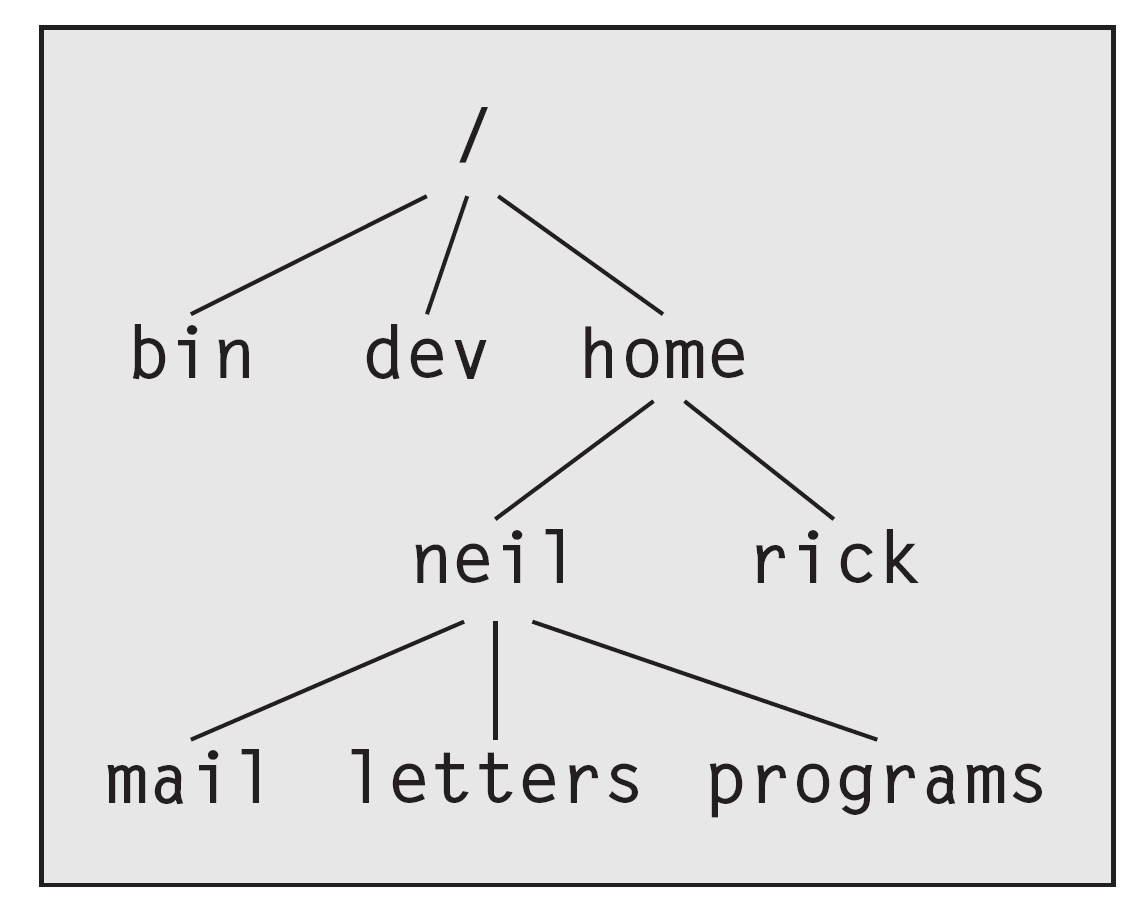
\includegraphics[width=1.0\textwidth]{../imgs/simple-directories.png}
\end{frame}

\begin{frame}{Constructor}
\begin{itemize}
\item Constructor
\begin{itemize}
\item place where you include code that initializes the object
\end{itemize}
\item Default Constructor
\begin{itemize}
\item no additional info required
\end{itemize}
\item User-defined Constructor
\begin{itemize}
\item with parameters that specify values or sizes
\end{itemize}
\item Java and C++ behave the same way with constructors
\end{itemize}
\end{frame}

\begin{frame}{Arrays}
\begin{itemize}
\item In Java arrays are actually objects that store length and other information.
\item In C++, an array is a sequence list of data. (Nothing else is stored.)

\item int x[20]; Button b[20];
\begin{itemize}
\item Valid declarations in C++, not in Java (why?)
\item Creates 20 ints and 20 Button objects
\end{itemize}
\end{itemize}
\end{frame}

\begin{frame}{Pointers and Arrays}
\begin{itemize}
\item In C++, there is a close relationship between pointers and arrays
\item Instead of int x[20]; can issue \\
int *x;  x = new int[20]; \\
to allow for dynamic allocation
\begin{itemize}
\item Usage of the array (e.g., x[3] = 5;) identical in both cases
\item To deallocate, use delete [] x;
\end{itemize}
\end{itemize}
\end{frame}

\begin{frame}{Constructors in Java and C++}
\begin{itemize}
\item In Java,
\begin{itemize}
\item a constructor is invoked only through the new keyword
\item recall that all object variables are references
\end{itemize}
\item In C++,
\begin{itemize}
\item a constructor is called upon variable declaration, or explicitly through new  with pointers, or in other situations
\item other types of constructors
\end{itemize}
\end{itemize}
\end{frame}

\begin{frame}{C++ Destructor}
\begin{itemize}
\item Special method whose signature is a ~ followed by the name of the class
\item e.g., ~SomeClass();
\item Particularly if the class contains pointers and the constructor contains calls to new, a destructor needs to be defined
\item e.g.,  SomeClass() { A = new int[20]; } \\
         ~SomeClass() { delete [] A; }
\end{itemize}
\end{frame}

\begin{frame}{C++ Control Over Copy and Assignment}
\begin{itemize}
\item In C++, the semantics of "a = b" (assignment) can be specified
\begin{itemize}
\item by defining the copy-assignment operator
\end{itemize}
\item In C++, there is a copy constructor
\begin{itemize}
\item specifies what happens during object copying, e.g., when function parameters are passed
\end{itemize}
\item There is more low-level control
\begin{itemize}
\item shallow copy vs deep copy
\end{itemize}
\end{itemize}
\end{frame}

\begin{frame}{Methods}
\begin{itemize}
\item Defines object behavior
\item Static methods vs instance methods
\item Method overloading
\begin{itemize}
\item within class, two methods with the same name but different signatures
\end{itemize}
\item Method overriding
\begin{itemize}
\item same signatures across different classes (subclass and superclass)
\end{itemize}
\end{itemize}
\end{frame}

\begin{frame}[fragile]{Operator Overloading}
\begin{itemize}
\item In C++, operators like =, +, *, ==, etc. can be defined, just like methods
\item Example:
\end{itemize}
\begin{lstlisting}
class Matrix {
   // ...
   Matrix operator+(Matrix m) { }//
} ;
c = a + b;  // equiv to c = a.operator+(b);
\end{lstlisting}
\end{frame}

\begin{frame}{Method Binding}
\begin{itemize}
\item Let Teacher be a subclass of Employee \\
\begin{itemize}
\item Also, suppose promote() is a method defined in both classes
\end{itemize}
\item Employee variables can refer to Teachers
\begin{itemize}
\item In Java, Employee e; e = new Teacher();
\item In C++, Employee *e; e = new Teacher;
\end{itemize}
\item e.promote() (or (*e).promote() ) calls which promote() method?
\end{itemize}
\end{frame}

\begin{frame}{Static vs Dynamic Binding}
\begin{itemize}
\item In C++, Employee's promote() is called
\begin{itemize}
\item Determined at compile time and deduced from the type of the variable (static binding)
\end{itemize}
\item In Java, Teacher's promote is called
\begin{itemize}
\item Determined at run-time because the actual type of the referred object is checked then (dynamic binding)
\end{itemize}
\end{itemize}
\end{frame}

\begin{frame}{There is more}
\begin{itemize}
\item While there are many more features I want to pause here before continuing
\end{itemize}
\end{frame}


\begin{frame}{homework}
\begin{itemize}
\item There is a lab \textbf{and} project assigned today
\item I recommend completing lab05 before starting the project.
\end{itemize}
\end{frame}

\end{document}
